\section{Simulation analysis}
\label{sec:simulation}

\subsection{Simulating the AC/DC converter for 10 periods}
As said in the introduction, the first step to this laboratory assignment was to simulate a simple AC/DC converter in NGSpice, the circuit features an ideal transformer, using a current controlled voltage source as well as a voltage controlled current source as explained by the professor in a previous lecture, as well as an envelope detector and a voltage regulator. \par
This AC/DC converter was simulated for 10 periods and all the analysis were made measuring on a $5e-5$ step in order to evaluate at least 1000 points during the 10 periods. In order to calculate this step we used the frequency of the AC source to know the period and then we multiplied this period by 10 in order to get the total time. We then divided the total time by 1000 points and made the step even smaller than that in order to make sure it had more than 1000 points but not too small that the program ran slowly. \par
This circuit was first made simple and was elaborated along the way, making it output the correct voltage, increasing the merit figure.

\subsection{Output voltage level}
After describing the circuit we made NGSpice measure the average output voltage and using a transient analysis we plotted both the average and the signal of the output voltage in the same graph. \par
The table and the graph below show the results we got.

\begin{table}[H]
  \centering
  \begin{tabular}{|l|r|}
    \hline    
    {\bf Name} & {\bf Value [V]} \\ \hline
    \input{average_tab}
  \end{tabular}
  \label{tab:average}
\end{table}

\begin{figure}[H] \centering
\includegraphics[width=0.7\linewidth]{../sim/transient1.pdf}
\caption{Plot of the average and the signal of the Output Voltage.}
\label{fig:transient1}
\end{figure}

\subsection{Output of the Envelope Detector and voltage Regulator circuits}
The output voltages of both the Envelope Detector as well as the Voltage Regulator circuits were plotted and put each in a different graph as well as a graph with both voltages plotted. \par
The three graphs are in the images below.

\begin{figure}[H] \centering
\includegraphics[width=0.7\linewidth]{../sim/transient2.pdf}
\caption{Envelope Detector Output Voltage.}
\label{fig:transient2}
\end{figure}

\begin{figure}[H] \centering
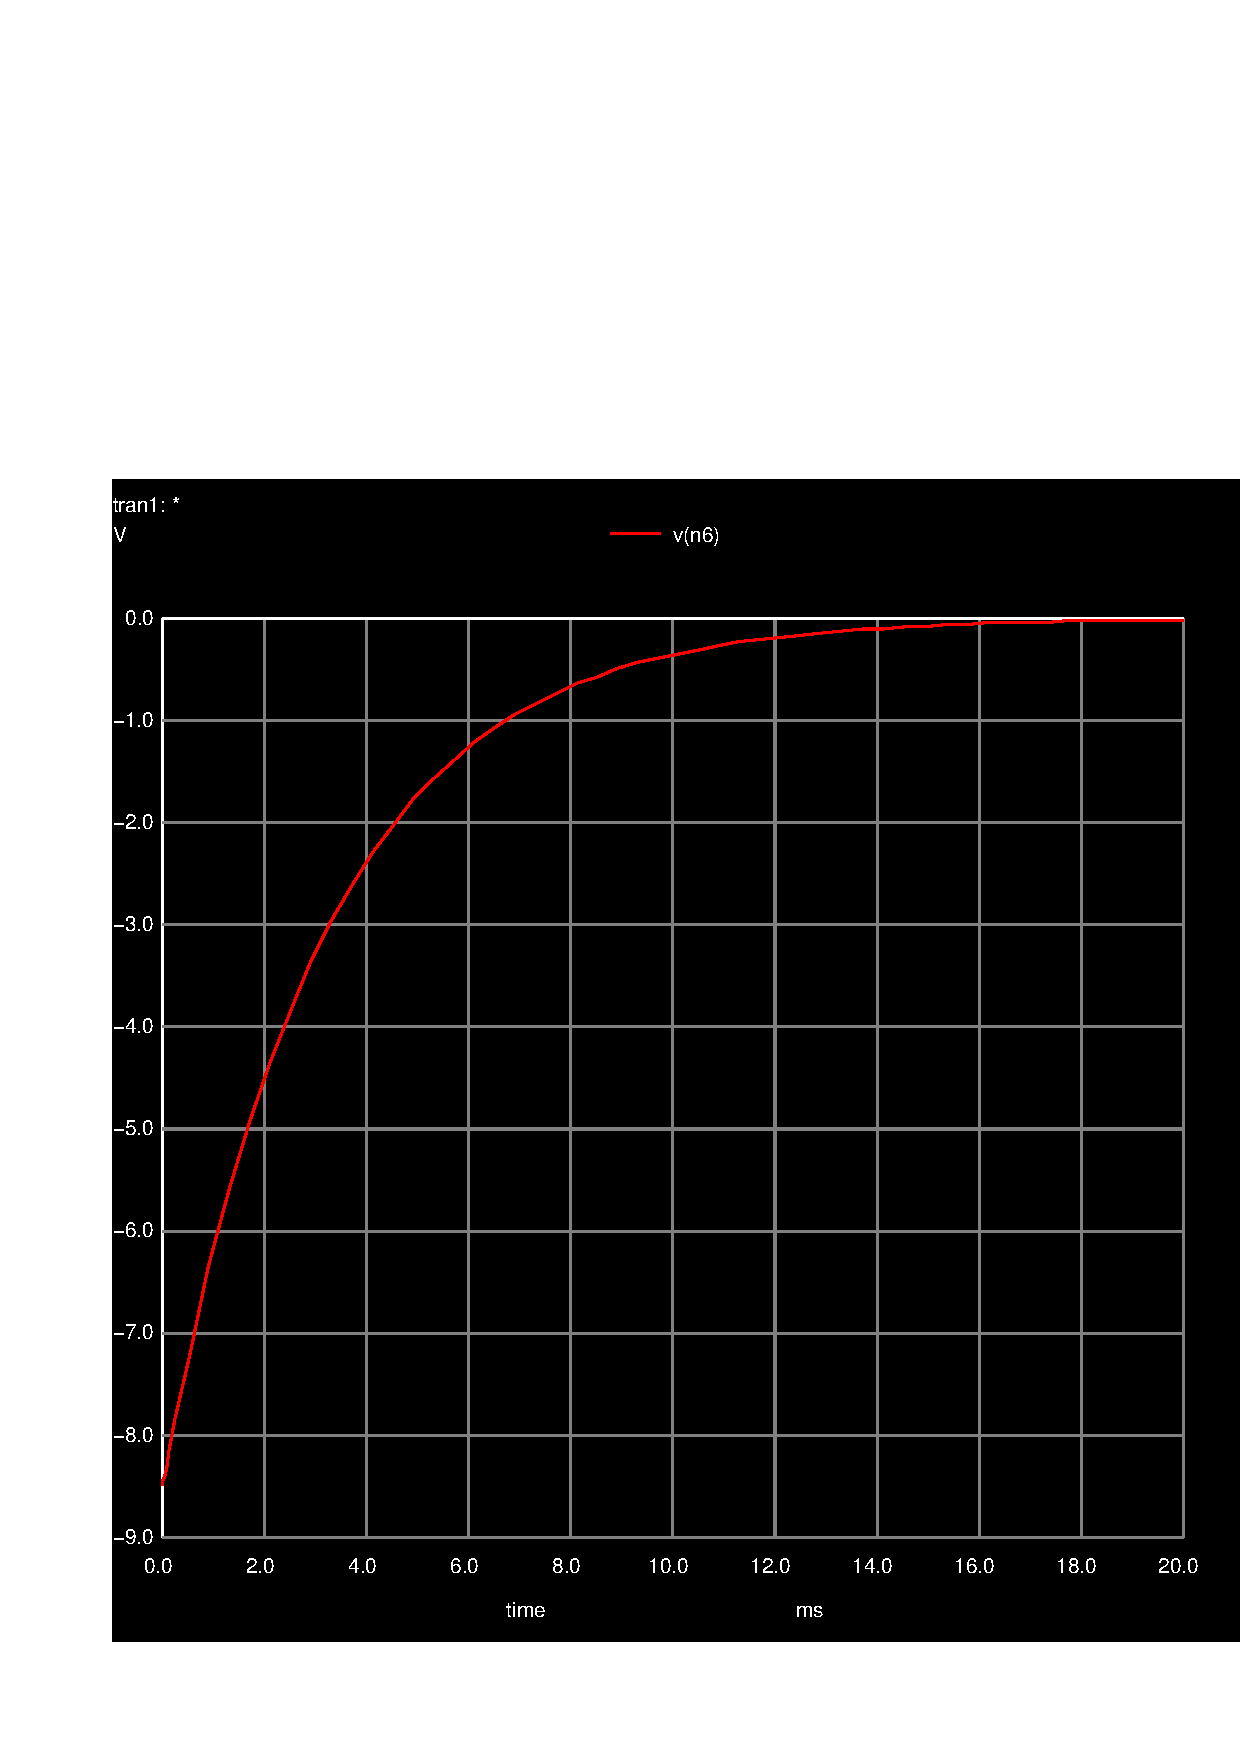
\includegraphics[width=0.7\linewidth]{../sim/transient3.pdf}
\caption{Voltage Regulator Output Voltage.}
\label{fig:transient3}
\end{figure}

\begin{figure}[H] \centering
\includegraphics[width=0.7\linewidth]{../sim/transient4.pdf}
\caption{Envelope Detector and Voltage Regulator Output Voltages.}
\label{fig:transient4}
\end{figure}

\subsection{Output voltage ripple}
We then made NGSpice measure the output voltage ripple, that is the difference between the maximum and the minimum values of the signal. \par
The result we got is in the table below.

\begin{table}[H]
  \centering
  \begin{tabular}{|l|r|}
    \hline    
    {\bf Name} & {\bf Value [V]} \\ \hline
    \input{ripple_tab}
  \end{tabular}
  \label{tab:ripple}
\end{table}

\subsection{$v_0 - 12$ plot}
Lastly, we plotted $v_0 - 12$, which corresponds to the output AC component plus the DC deviation. \par
The plot can be seen in the image below.

\begin{figure}[H] \centering
\includegraphics[width=0.7\linewidth]{../sim/transient5.pdf}
\caption{Output AC component + DC deviation.}
\label{fig:transient5}
\end{figure}




